\documentclass[10pt]{report}

\title{Teknologiprosjekt: Øving 1}
\author{Mathias Mellemstuen}
\date{17.09.20}

\DeclareFixedFont{\ttb}{T1}{txtt}{bx}{n}{10} % for bold
\DeclareFixedFont{\ttm}{T1}{txtt}{m}{n}{10}  % for normal
\usepackage[margin=1in]{geometry}
\usepackage{color}
\usepackage{graphicx}
\usepackage{listings}
\usepackage{wrapfig}
\usepackage{amsmath}

\definecolor{light}{rgb}{0.5, 0.5, 0.5}
\def\lighterText#1{{\color{light}#1}}
\definecolor{deepblue}{rgb}{0,0,0.5}
\definecolor{deepred}{rgb}{0.8,0,0}
\definecolor{deepgreen}{rgb}{0,0.5,0}
\definecolor{grey1}{rgb}{0.5,0.5,0.5}


% Python style for highlighting
\newcommand\pythonstyle{\lstset{
		language=Python,
		basicstyle=\tiny\ttm,
		otherkeywords={self},             % Add keywords here
		keywordstyle=\tiny\ttb\color{deepblue},
		emph={},          % Custom highlighting
		emphstyle=\tiny\color{deepred},    % Custom highlighting style
		stringstyle=\tiny\color{deepgreen}\ttm,
		commentstyle=\tiny\color{grey1}\ttm,
		frame=none,                         % Any extra options here
		showstringspaces=false,            % 
		breaklines=true,
		tabsize=2
}}
% Python environment
\lstnewenvironment{python}[1][] {
	\pythonstyle
	\lstset{#1}
}{}

% Python for external files
\newcommand\pythonexternal[2][]{{
		\pythonstyle
		\lstinputlisting[#1]{#2}}}

% Python for inline
\newcommand\pythoninline[1]{{\pythonstyle\lstinline!#1!}}

\newcommand{\Vi}{\vec{i}}

\begin{document}
\begin{flushright}
\lighterText{Mathias Mellemstuen (17.09.20)}
\end{flushright}
\begin{center}
\section*{Teknologiprosjekt: Øving 1}
\textbf{Robotarium experiment with motion planning and control}
\line(1,0){400}
\end{center}
The undertaken task was to design, simulate, test and implement a simple motion planning and control algorithm. The motion control algorithm should be written in Python and tested on the Robotarium robotics simulator.
Python code can be deployed on a real robot when the code is thoroughly tested with the Robotarium simulator.
The robot should follow a track which resembles the shape of the infinity symbol.
\\\\
\textbf{Creating the Infinity track}\\
Since the robot in this case always know it's current (x,y) coordinates and angular rotation at all times,
it would make sense to store the track as an array of (x,y) coordinates and then use trigonometry to find
the distance and angle between the robot and the current waypoint.The array with all the coordinates can then be two-dimentional and defined like this: 
\begin{python}
path = [
    [0.0, ...], # Array with x coordinates
    [0.0, ...]  # Array with y coordinates
]
\end{python}
The Robatarium API has a function that allows you to plot lines between points. This function can be used to draw the track with the path variable. 
\begin{python}
# Plotting a red line between the points in the path. 
def plotTrack():
    r.axes.plot(path[0],path[1],color='red',linewidth = lineWidth)
\end{python}
Since the edges of the infinity symbol is circular, it will also need a way to plot points in a circle:
\begin{python}
# Normalizing a value between min - max
def normalize(min, max, value): 
    return min + (max - min) * value 

# Creating a part of a circle fromRadians -> toRadians
def createCircle(x, y, fromRadians, toRadians, step, normalizeMin, normalizeMax): 
    current = fromRadians
    circle = [[],[]]
    while(current < toRadians):
        circle[0].append(x + normalize(normalizeMin, normalizeMax, math.cos(current)))
        circle[1].append(y + normalize(normalizeMin, normalizeMax, math.sin(current)))
        current += step
return circle
\end{python}
\begin{minipage}[r]{0.5\textwidth}
Now it's possible to hardcode the straight lines and then use the \pythoninline{createCircle} function to create the curved part of the infinity symbol, then append everything in the right order to \pythoninline{path}.
The end results after doing this looks like this.
\end{minipage}
\begin{minipage}[l]{0.5\textwidth}
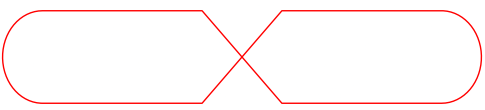
\includegraphics[width=\linewidth]{infinitypicture.png}
\end{minipage}
. \\
\textbf{Motion control algorithm} \\
There is many ways of approaching this problem. It can be done relativly simple since we are not considereing collision detection and the robot does always have track of it's position and it's current waypoint position.
Because of this, we only need an algorithm that calculates vertical and angular velocity of the robot so the robot moves towards the current waypoint. When the robot then has approached an acceptable distance to the current waypoint, then change to the next waypoint in the path and run the algorithm again. 
This can be represented in an algorithm like this: 
\begin{enumerate}
    \item When the robot is within an acceptable distance to the current waypoint (n), change the current waypoint to (n+1).
    \item Calculate the current distance and the angle between the robot and the waypoint. The distance between the robot and the target can be calculated with the pythagoras sentence, $\alpha = \sqrt{\Delta x^{2} + \Delta y^{2}}$.
    The equation can be written like this in python: 
    \begin{python}
def calculateDistanceBetweenTwoPoints(x1,y1,x2,y2):
    return math.sqrt(math.pow(x2 - x1,2) + math.pow(y2 - y1, 2))
    \end{python}
    The shortest angle in radians between the robot and the waypoint can be defined like this: $\alpha = atan2(\Delta y, \Delta x)$.
    This can be translated to this python function:
    \begin{python}
def calculateAngleBetweenPoints(x1,y1,x2,y2):
    deltaX = x2 - x1
    deltaY = y2 - y1
    return math.atan2(deltaY, deltaX)
    \end{python}    
    \item It's now possible to calculate the shortest way to turn the robot (left/right), so the robots facing angle goes towards the angle between the robot and the waypoint. This can be done with this python function: \begin{python}
def shortestWayBetweenTwoAngles(angle1, angle2): 
    angle1 = float(angle1)
    angle2 = float(angle2)

    if angle1 < angle2 and angle2 - angle1 <= math.pi:
        return 1.0
    if angle1 < angle2 and angle2 - angle1 > math.pi:
        return -1.0
    if angle1 > angle2 and angle1 - angle2 <= math.pi:
        return -1.0
    if angle1 > angle2 and angle1 - angle2 > math.pi:
        return 1.0

    return 0.0
    \end{python} The return value of this function is 1 if the most efficient way to turn is right, -1 for left and 0 if the angles are the same. 
    \item Calculate the robots next velocities based on how far away it's from the current waypoint and how far off it's angle is. 
    \begin{python}
def calculateNextVelocity(position):
    
    global currentTarget

    targetX = path[0][currentTarget]
    targetY = path[1][currentTarget]

    distanceToTarget = calculateDistanceBetweenTwoPoints(targetX,targetY,position[0],position[1])    
    
    currentTarget = currentTarget if not (distanceToTarget < acceptableDistanceToTarget) else (currentTarget + 1) if (currentTarget is not len(path[0]) - 1) else 0

    targetX = path[0][currentTarget]
    targetY = path[1][currentTarget]

    targetAngle = convertAngle0To2Pi(calculateAngleBetweenPoints(position[0], position[1], targetX, targetY))
    angle = convertAngle0To2Pi(position[2])

    speed = maxSpeed - calculateSpeedModifierBasedOnAngleDifferenceAndDistance(angle, targetAngle, distanceToTarget)
    if speed < 0: speed = 0
    
    setVelocity(speed,0 if calculateAngleDifference(angle, targetAngle) < acceptableAngleError else turningSpeed * shortestWayBetweenTwoAngles(angle, targetAngle))
    \end{python}
    \item The velocity can then be applied to the robot. These 5 steps will be repeated until the code is terminated. 
    \begin{python}
def robotLogic():
    position = r.get_poses()
    calculateNextVelocity(position)
    v = velocity
    v.shape = (2,1)
    r.set_velocities(numberOfRobots, v)
    r.step()

while running: robotLogic()
    \end{python}
\end{enumerate}
\textbf{Results of the simulation} \\
The robot worked very good in the simulation. It didn't overshoot much and manages to stay on the red line at all times while driving relatively fast. It manages to stay on the course by decreasing it's linear velocity if the turn becomes too steep. It is possible that it could be faster if for instance lookahead was implemented in the algorithm. Then it could take more than just the current waypoint into consideration, and that would probably optimize it more.
\\\\
\textbf{Results of the algorithm deployed on a real robot} \\
The code worked while being deployed on a real robot, but the quality was worse than in the simulation. It did move slower around the course and it had to completely stop sometimes to turn to correct it's angular error.
\end{document}
